\documentclass[10pt,letterpaper]{article}

\usepackage{kpfonts}
\usepackage{kpfonts}
\usepackage[utf8]{inputenc}
\usepackage[T1]{fontenc}
% \usepackage{fancyhdr}
\usepackage{natbib}
\usepackage{booktabs}
\usepackage{longtable}
\usepackage{multirow}
\usepackage{graphicx}
\usepackage{siunitx}
\usepackage[pdftex, hidelinks, bookmarks=true, bookmarksopen=true]{hyperref}
\usepackage{doi}
\usepackage[hmargin=2.5cm,vmargin=2.5cm]{geometry}

\usepackage[usenames,dvipsnames]{color}
\definecolor{amber}{rgb}{1.0, 0.75, 0.0}
\definecolor{deeppink}{rgb}{1.0, 0.08, 0.58}
\definecolor{modblue1}{rgb}{0.0627, 0.3059, 0.4902}
\definecolor{modblue2}{rgb}{0.0824, 0.3961, 0.6235}
\definecolor{modblue3}{rgb}{0.2706, 0.6235, 0.7686}
\definecolor{modgray}{rgb}{0.2, 0.2, 0.2}
\definecolor{modgreen}{rgb}{0.18039216, 0.49019608, 0.19607843}
\newcommand{\clink}[2]{{\color{modblue2} \href{#1}{#2}}}

\usepackage{listings}
\lstset{language=sh,basicstyle={\bfseries \color{modgreen}},keywordstyle={\bfseries \color{modgreen}}}

% \setlength\parskip{0.8em plus 0.1em minus 0.2em}
% \setlength\parindent{0pt}
\usepackage{parskip}

\usepackage{fancyvrb}
\DefineVerbatimEnvironment{verbatim}{Verbatim}{xleftmargin=.1in}




\title{BLT Mooring Data Processing Notes}
\author{Gunnar Voet}


\begin{document}
\maketitle

The processing code and source code for this document are hosted on \clink{https://github.com/gunnarvoet/blt-proc}{GitHub}.

\section*{Mooring Narrative}
\label{sec:mooring_operations}

Mooring MP1 was deployed for only a few days during the BLT1 cruise in 2021.
Moorings MP1, MAVS1, MAVS2, and the TCHAIN mooring were deployed during BLT1.
MAVS1, MAVS2, and MP2 were recovered during BLT2 and redeployed as MAVS3, MAVS4, and MP3.
They were recovered during BLT3, together with the TCHAIN.
Two small moorings, G1 and LANDER, were deployed for only a few days during BLT3.
Mooring locations are shown in Figure~\ref{fig:mooring_map} and Table~\ref{tab:moorings}.

\begin{longtable}{p{1.7cm}p{2.3cm}p{2.3cm}p{2.3cm}p{2.3cm}p{1.3cm}}
\caption{BLT mooring deployment periods and locations.}
\label{tab:moorings}\\
\toprule
Mooring & Deployed & Recovered & Latitude & Longitude & Bottom Depth\\
\midrule
\endfirsthead
\caption[]{BLT mooring deployment periods and locations.} \\
\toprule
Mooring & Deployed & Recovered & Latitude & Longitude & Bottom Depth\\
\midrule
\endhead
\midrule
\multicolumn{2}{r}{{Continued on next page}} \\
\midrule
\endfoot

\bottomrule
\endlastfoot
MP1     & 2021-06-28 & 2021-07-05 & 54$^{\circ}$\,14.312'\,N & 11$^{\circ}$\,56.923'\,W & 2035\,m \\
MP2     & 2021-07-07 & 2021-10-05 & 54$^{\circ}$\,12.211'\,N & 11$^{\circ}$\,52.376'\,W & 1676\,m \\
MP3     & 2021-10-22 & 2022-08-02 & 54$^{\circ}$\,11.122'\,N & 11$^{\circ}$\,50.788'\,W & 1491\,m \\
MAVS1   & 2021-07-06 & 2021-10-05 & 54$^{\circ}$\,11.849'\,N & 11$^{\circ}$\,51.719'\,W & 1614\,m \\
MAVS2   & 2021-07-07 & 2021-10-04 & 54$^{\circ}$\,10.938'\,N & 11$^{\circ}$\,50.572'\,W & 1465\,m \\
MAVS3   & 2021-10-22 & 2022-08-04 & 54$^{\circ}$\,10.993'\,N & 11$^{\circ}$\,51.089'\,W & 1434\,m \\ 
MAVS4   & 2021-10-22 & 2022-08-08 & 54$^{\circ}$\,11.231'\,N & 11$^{\circ}$\,50.584'\,W & 1455\,m \\
TCHAIN  & 2021-07-06 & 2022-08-10 & 54$^{\circ}$\,11.413'\,N & 11$^{\circ}$\,51.137'\,W & 1529\,m \\
LANDER  & 2022-08-02 & 2022-08-10 & 54$^{\circ}$\,13.262'\,N & 11$^{\circ}$\,54.907'\,W & 1857\,m \\
G1      & 2022-08-04 & 2022-08-10 & 54$^{\circ}$\,10.296'\,N & 11$^{\circ}$\,49.767'\,W & 1281\,m \\

\end{longtable}


Further details on mooring operations can be found in the cruise reports.

\section*{Software Environment}
\label{sec:software_environment}

Some of the Python processing files were written as Jupyter notebooks and converted to python scripts using \clink{https://jupytext.readthedocs.io/en/latest/}{jupytext}. They can be converted back to Jupyter notebooks.

A \clink{https://docs.conda.io/en/latest/}{conda} environment with all packages needed for running the python processing scripts can be created by running \lstinline{conda env create -f environment.yml}. The newly created environment will be called \lstinline{blt-proc}.


\begin{figure}[htpb]
    \centering
    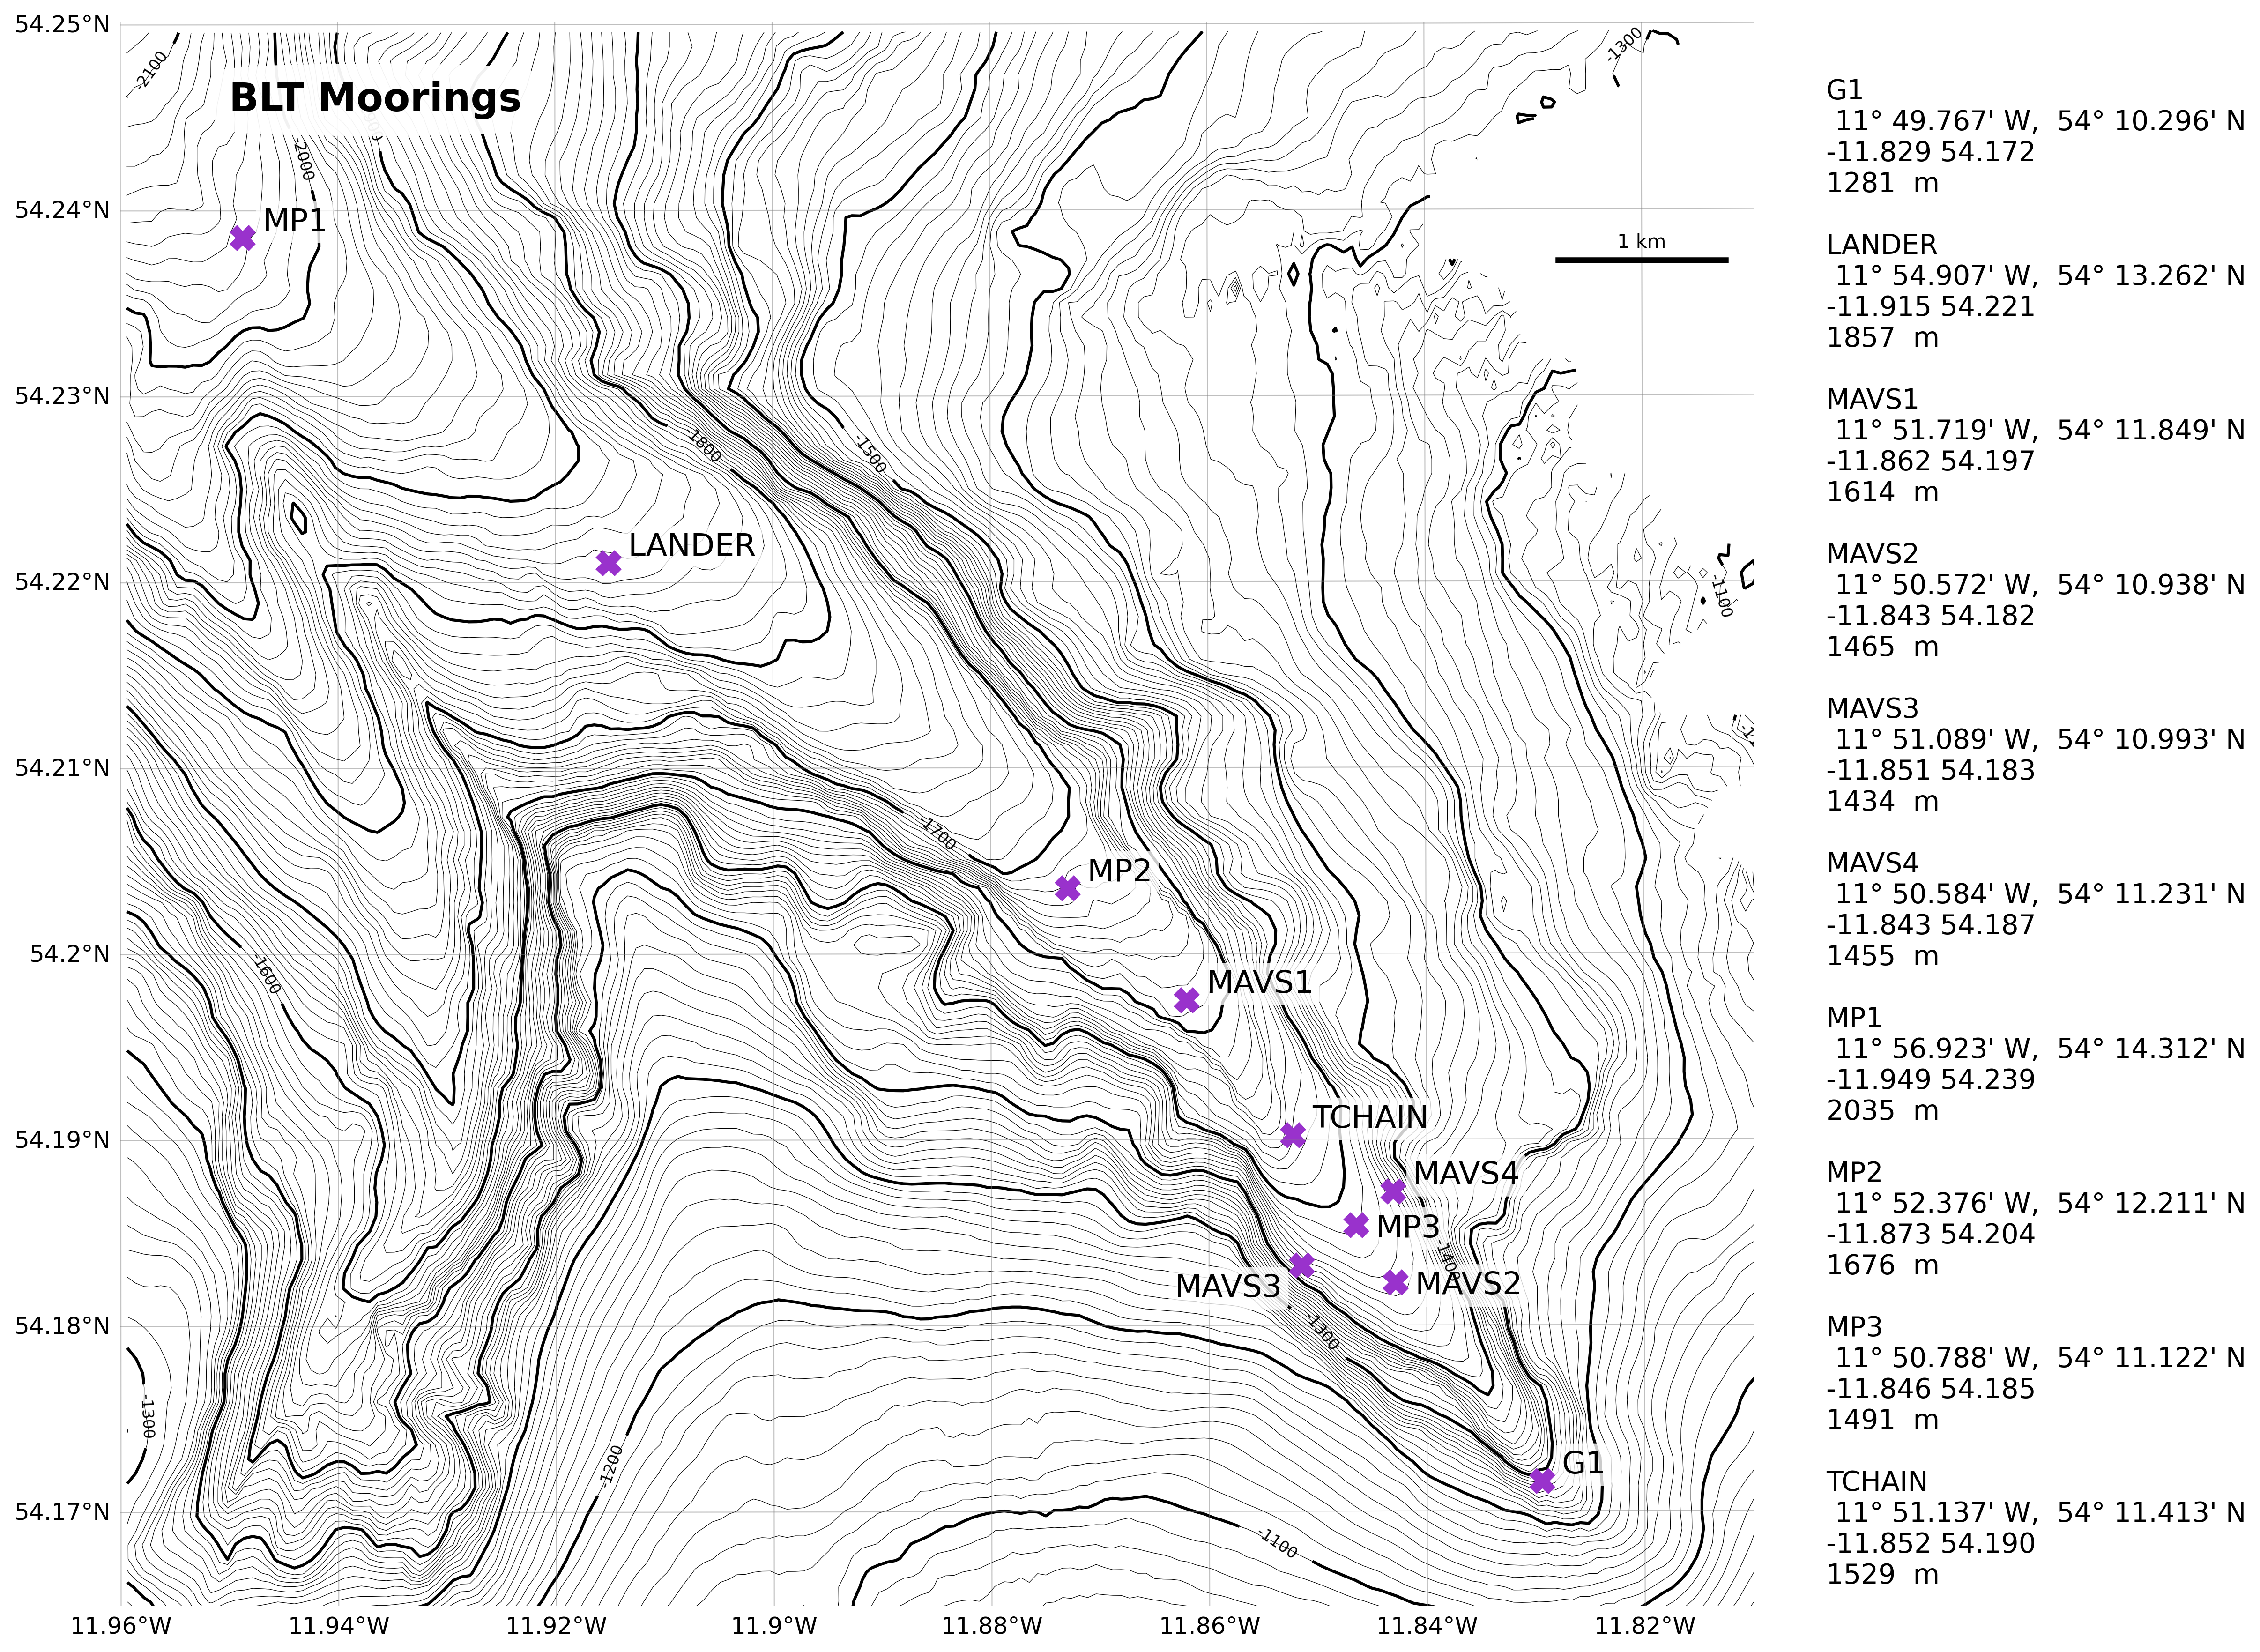
\includegraphics[width=\textwidth]{fig/blt_mooring_locations.png}
    \caption{Mooring locations inside the Rockall Trough Canyon.}
    \label{fig:mooring_map}
\end{figure}


The \lstinline{Makefile} bundles a number of data synchronization and processing steps.
Note that GNU \lstinline{make} version 4.3 or higher is necessary for this to work properly.
Under macOS, this can be installed via \lstinline{brew install make} using \clink{https://brew.sh/}{homebrew}.
Type \lstinline{make help} to see various options for running the Makefile.

\section*{ADCP}
\label{sec:adcp}

Magnetic declination at the mooring sites is about -5 and determined running \lstinline{magdec} inside \lstinline{gadcp}.


\section*{SBE37}
\label{sec:sbe37}


CTD rosette calibration prior to BLT2 mooring deployments on 2021-10-15 (cast 73).


\section*{Thermistors}
\label{sec:thermistors}

\subsection*{SBE56}
\label{sec:sbe56}

\subsubsection*{BLT1}
\label{sub:sbe56_blt1}
All SBE56 sampled at 2\,s period or 0.5\,Hz during BLT1 with the exception of SN\,455. This instrument reset shortly after deployment and then sampled at 0.5\,s period or 2\,Hz.

Two of the thermistors (466, 6424) had pretty severely bent probes due to impact on prior deployments. Their time series and variance spectra look fine though.

We performed warm water dips prior to and after deployment to calibrate the instrument clocks. After applying time drift offsets as determined on data download, the spike in temperature from the water bath lines up with shipboard UTC time. In one case (455) the clock had reset shortly after the beginning of the deployment and the signal from the warm water dip was used to generate a time vector.

Some of the instruments exhibit short gaps in the time series. These are marked in table~\ref{tab:sbe56}. Gaps are much shorter than 1 hour.

Some instruments started dropping out prior to recovery. Most of them show events (Power on Reset / Power Fail Reset) in their logs.

Data have been processed to level 0 (only converted, no corrections applied except for clock drift) and level 1 (cut to time at depth without including gaps in the data longer than 1~hour, CTD calibration offset applied).

\subsubsection*{BLT2}
\label{sub:sbe56_blt2}

Overall performance was much better for the BLT2 deployment compared to BLT1. Sampling period was set to 8s.

Table~\ref{tab:blt2_sbe56} lists notes from data download and processing. Only two loggers (915, 916) terminated early. SN418 showed a few seconds departure from the clock calibration, most likely due to a wrong time noted on data downloaded. This has been corrected for. SN6445 has been lost.

Data processing followed the procedure outlined for BLT1 SBE56s. We used the same CTD calibration offsets from the cast in October 2021.


\subsubsection*{SBE56 CTD Calibration}
\label{sub:sbe_ctd_calibration}

All SBE56 were attached to the CTD rosette after BLT1 recoveries during the second cruise. Thermistor time series from the CTD cast are thus separate from the BLT1 deployment. Figure~\ref{fig:sbe56_ctd_cal_photo} shows the thermistors physically mounted on the rosette near the vane. Unfortunately, the sensors were set to sample only every 60\,s during the CTD calibration cast. The rosette stop near the bottom still provides at least one calibration point and sensor offsets were determined. Figure~\ref{fig:sbe56_ctd_cal} shows the CTD and thermistor time series near the bottom at around 4.6$^{\circ}$C in-situ temperature. Offsets are generally within 2~millidegrees of the CTD temperature sensor~1. The offsets are subtracted from the thermistor time series in the level~1 dataset.

\begin{figure}[htpb]
    \centering
    \includegraphics[width=0.6\linewidth]{fig/blt2_sbe56_solo_calibration.jpg}
    \caption{SBE56 mounted for CTD calibration cast near the rosette vane during BLT2. RBR Solos were mounted as well for a pre-deployment calibration cast.}
    \label{fig:sbe56_ctd_cal_photo}
\end{figure}

\begin{figure}[htpb]
    \centering
    \includegraphics[width=0.7\linewidth]{fig/blt1_sbe56_ctd_cal_bottom.png}
    \caption{SBE56 CTD cal bottom time series. CTD temperature time series are shown in blue and orange for CTD sensors 1 and 2, all SBE56 time series are shown in gray with dots marking data points every 60s.}
    \label{fig:sbe56_ctd_cal}
\end{figure}



\subsection*{RBR Solo}
\label{sec:rbr_solo}

\subsubsection*{BLT1}
\label{sub:rbr_blt1}
% Some of the processing code lives in a separate repository at \clink{https://github.com/gunnarvoet/rbrmoored}{rbrmoored}.
RBR Solo time series were processed without any major issues. The newly delivered units died early for at this point still unknown reasons. Table~\ref{tab:rbrsolo} lists all sensor that had issues.

We performed warm water dips prior to and after deployment to calibrate the instrument clocks. After applying time drift offsets as determined on data download, the spike in temperature from the water bath lines up with shipboard UTC time. This clock verification could not be carried out for the instruments listed in table~\ref{tab:rbrsolo}. Cross-correlation functions calculated from neighboring instruments do not indicate any major time drift on these units.
  
\subsubsection*{BLT1 RBR Solo CTD Calibration}
\label{sub:blt1_rbr_ctd_calibration}
All RBR Solo were attached to the CTD rosette prior to the BLT1 deployment.
Calibration casts were done on 2021-06-22 and 2021-06-23, corresponding to CTD casts 002 and 003. Cast 003 was deeper than 1700m and the plastic (WHOI) RBRs were taken off for this cast. Figure~\ref{fig:blt1_rbr_calibration} shows some of the sensors physically mounted on the rosette for CTD cast~002.

\begin{figure}[htpb]
    \centering
    \includegraphics[width=0.6\linewidth]{fig/blt1_rbr_calibration.jpg}
    \caption{RBR thermistors mounted for CTD calibration cast during BLT cruise 1 (CTD cast 002).}
    \label{fig:blt1_rbr_calibration}
\end{figure}

\begin{figure}[htpb]
    \centering
    \includegraphics[width=0.7\linewidth]{fig/blt1_rbr_ctd_cal_cast_20210622.png}
    \includegraphics[width=0.7\linewidth]{fig/blt1_rbr_ctd_cal_cast_20210623.png}
    \caption{Two RBR CTD calibration casts (002 and 003). Red parts of the pressure time series mark calibration stops referred to in figures~\ref{fig:rbr_ctd_cal_stops_cast2} and~\ref{fig:rbr_ctd_cal_stops_cast3}.}%
    \label{fig:fig/rbr_ctd_cal_casts_overview}
\end{figure}

\begin{figure}[htpb]
    \centering
    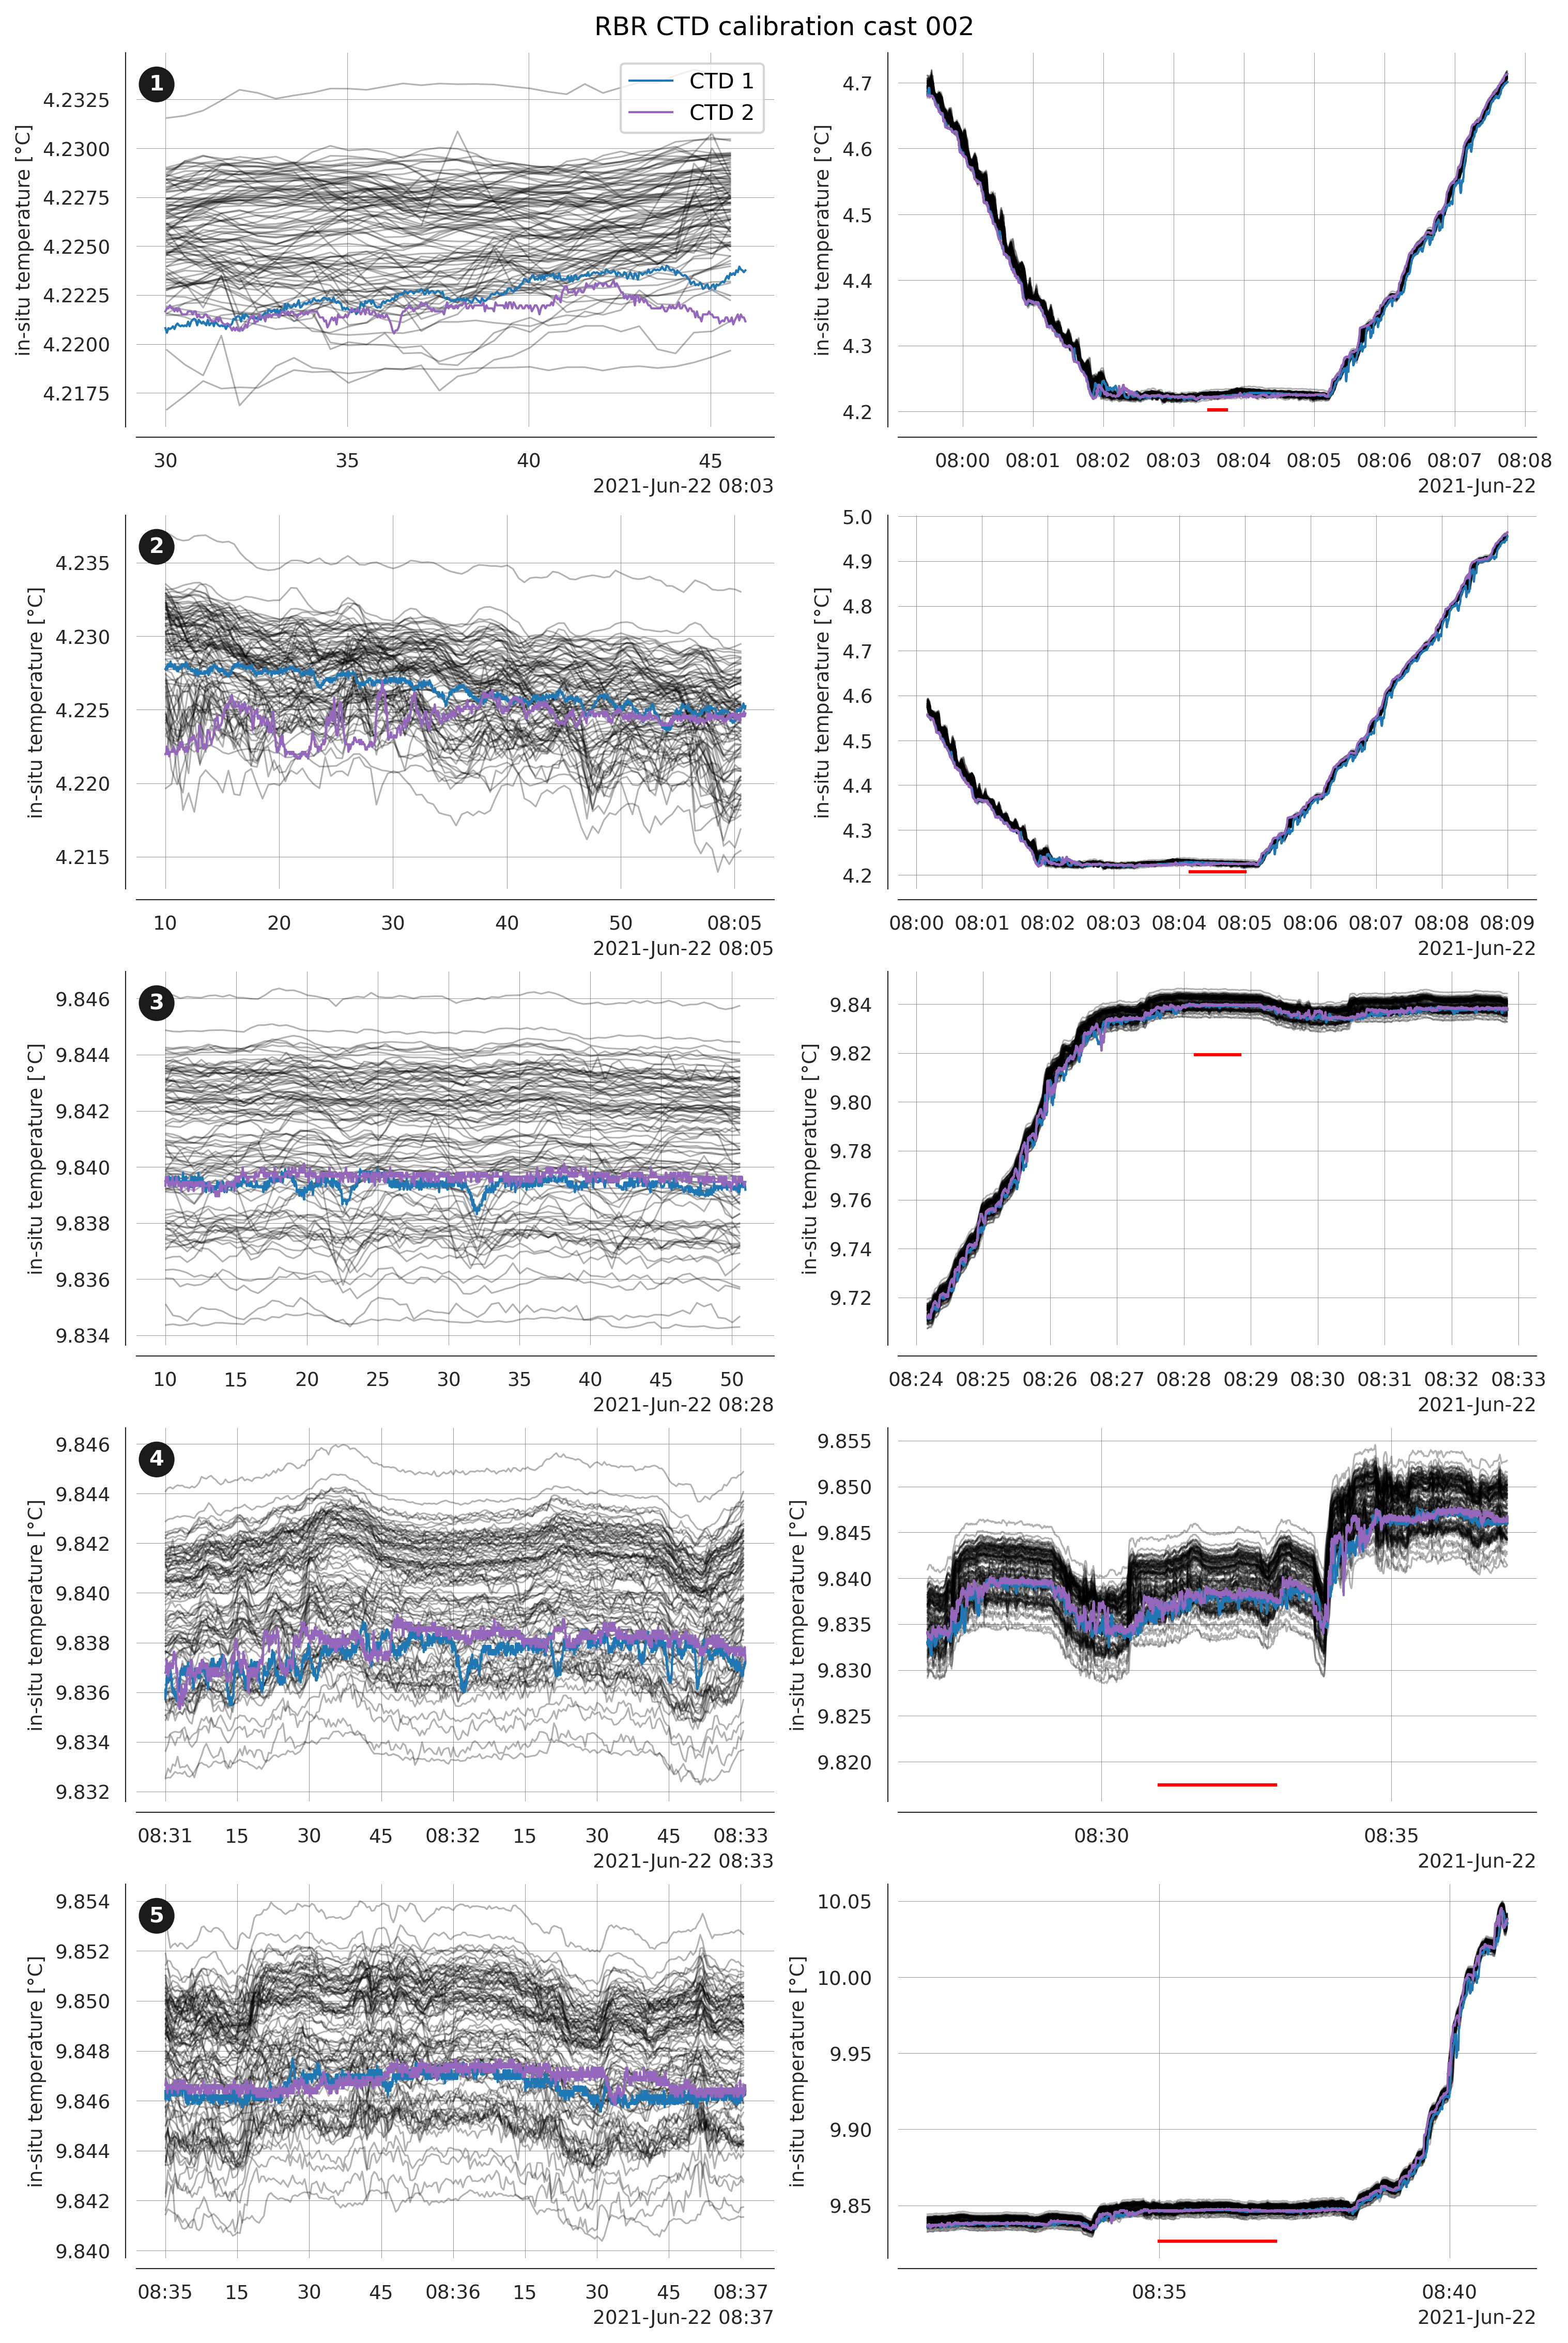
\includegraphics[width=0.9\linewidth]{fig/blt1_rbr_ctd_cal_cast_002_stops.png}
    \caption{CTD cast 002 calibration stops.}%
    \label{fig:rbr_ctd_cal_stops_cast2}
\end{figure}

\begin{figure}[htpb]
    \centering
    \includegraphics[width=0.9\linewidth]{fig/blt1_rbr_ctd_cal_cast_003_stops.png}
    \caption{Cast 003 calibration stops.}%
    \label{fig:rbr_ctd_cal_stops_cast3}
\end{figure}

Cast 002 did not go all the way to the bottom (had to stop earlier due to the 1700\,m rated instruments). Unfortunately, the deep stop around 4.2$^{\circ}$C shows lots of variability and doesn't provide a good calibration point. Figure~\ref{fig:rbr_ctd_cal_stops_cast2} shows two short chunks of this stop in panels 1 and 2. The stops higher up at around 9.8$^{\circ}$C are more stable and provide reliable calibration data.

Cast 003 has a very stable period at the bottom (Fig.~\ref{fig:rbr_ctd_cal_stops_cast3} panel~2. Offsets determined here are within a few millidegrees for most sensors. Only 3 deep Solos differ by more than 5 millidegrees: 72147 (6mdeg), 72216 (-12mdeg), 72219 (-6mdeg). Cast 003 has stops at 1500m and 300m in addition to the bottom stop.

We do not have enough data to fit a polynomial to the calibration points. Maybe the best we can do is determine a constant offset from the points we have. We use points 3~to~5 on cast~002 and points 2~to~4 on cast 003 to calculate a mean offset for each thermistor.

72216 shows a bit of a funky behavior in the calibration where the offset seems to linearly increase with temperature. We may want to apply a linear fit to the calibration data instead of just computing a constant offset, this has not been implemented yet.

\subsubsection*{BLT1 RBR Solo MAVS}
\label{sub:blt1_rbr_solo_mavs}
Reading the thermistor data from Kurt's processed .mat-files. The time series do not have the clock drift applied. Kurt provides the clock readings after recovery in his little write-up on the MAVS data. Clocks are corrected in the level 0 and level 1 datasets for these units. Cross-correlation with neighboring thermistors indicates good clocks, i.e.~no significant lag between signals is detected. 


\subsubsection*{BLT2}
\label{sub:rbr_blt2}
102986 appears to have been lost.

102974 terminates early in Feb 2022.
202307 appears to broken starting in mid-December.

\subsubsection*{BLT2 RBR Solo CTD Calibration}
\label{sub:blt2_rbr_ctd_calibration}

During BLT2 the CTD rosette calibration happened either on Oct 13 around 16:00 (cast~62) or Oct 15 around 15:00 (cast~72). These CTD casts have been processed by Gunnar using the Python \clink{https://ctdproc.readthedocs.io/en/latest/}{ctdproc} package.

102974 was not included in the CTD calibration. Maybe we can use the BLT1 calibration. Also no data for 202304, 202305, 202306, 202307. And possibly for some of the time series that I still need to get from Kurt.

\subsubsection*{BLT2 RBR Solo MAVS}
\label{sub:blt2_rbr_solo_mavs}
For thermistors that had been integrated with MAVS-sensors, time drift was determined by correlating 3-day-long time series with neighboring sensors where the clock is known to be good. The clock correction has been applied to these sensors in the level 1 time series.

\clearpage
\begin{longtable}{p{1.5cm}p{10cm}}
\caption{RBR Solo processing notes. The major issue was the early battery termination on all newly delivered thermistors. At the time of data processing the exact reason for the short lived batteries remains unclear.}
\label{tab:rbrsolo}\\
\toprule
{} &                                        Processing Notes \\
SN     &                                                         \\
\midrule
\endfirsthead
\caption[]{RBR Solo processing notes. The major issue was the early battery termination on all newly delivered thermistors. At the time of data processing the exact reason for the short lived batteries remains unclear.} \\
\toprule
{} &                                        Processing Notes \\
SN     &                                                         \\
\midrule
\endhead
\midrule
\multicolumn{2}{r}{{Continued on next page}} \\
\midrule
\endfoot

\bottomrule
\endlastfoot
72183  &                     large time offset (seems ok though) \\
72188  &  time series terminating early; no time offset recorded \\
207286 &  time series terminating early; no time offset recorded \\
207287 &  time series terminating early; no time offset recorded \\
207288 &  time series terminating early; no time offset recorded \\
207289 &  time series terminating early; no time offset recorded \\
207300 &  time series terminating early; no time offset recorded \\
207301 &  time series terminating early; no time offset recorded \\
207302 &  time series terminating early; no time offset recorded \\
207303 &  time series terminating early; no time offset recorded \\
207304 &  time series terminating early; no time offset recorded \\
207305 &  time series terminating early; no time offset recorded \\
207306 &  time series terminating early; no time offset recorded \\
207307 &  time series terminating early; no time offset recorded \\
207308 &  time series terminating early; no time offset recorded \\
207309 &  time series terminating early; no time offset recorded \\
207375 &  time series terminating early; no time offset recorded \\
207376 &  time series terminating early; no time offset recorded \\
207377 &  time series terminating early; no time offset recorded \\
207378 &  time series terminating early; no time offset recorded \\
207379 &  time series terminating early; no time offset recorded \\
207380 &  time series terminating early; no time offset recorded \\
207381 &  time series terminating early; no time offset recorded \\
207382 &  time series terminating early; no time offset recorded \\
207383 &  time series terminating early; no time offset recorded \\
\end{longtable}


\subsection*{Thermistor In-Situ Calibration}
\label{sec:thermistor_in_situ_calibration}

In addition to the CTD calibration casts, thermistors are also calibrated in-situ by comparison with mean temperature stratification calculated over two-day windows. An inertial period is about 0.6 days at the mooring sites, we are thus averaging over enough time to expect stable stratification.

Expand a bit more here on \citet{cimatoribusetal16}.

\section*{Mooring Trilateration}
\label{sec:trilateration}
The bulk of the trilateration processing code now lives in \clink{https://github.com/gunnarvoet/gvpy}{gvpy} under \lstinline{gvpy.trilaterate}. Survey setup for MAVS2 and MP2 was such that the software does not determine the right position from the three-point solution and the average of the two-point solutions was chosen instead.


\section*{Multibeam}
\label{sec:multibeam}
There seems to be a bug in \lstinline{mbgrid} such that if the option \lstinline{-U} [time] is not set then only very few data points are used in the processing. Now providing a time parameter that incorporates six months such that all data should be included.

Also now outputting the number of data points and standard deviation per grid cell via \lstinline{-M}.

Now setting minimum velocity to \qty{1}{km/h} to get rid of some of the stationary data that are noisier.

\section*{Appendix: Thermistors}
\label{sec:appendix_thermistors}

\subsubsection*{BLT1 SBE56 Instrument Issues}
\label{ssub:blt1_sbe56_instrument_issues}
Some sensor specific information below for thermistors that did not perform as expected.

\paragraph{High Current Sensors}
The following thermistors had 62 "Events" and are possibly high current.
\begin{itemize}
    \item 0392 (Ended Late Sept 2.75 month duration)
    \item 0413 (Ended Late Sept 2.75 month duration)
    \item 0421 (Ended Early Sep 2 month duration)
    \item 0423 (Ended Mid Sept 2.5 month duration)
    \item 0425 (Ended Late Sept 2.75 month duration)
    \item 0915 (Ended Late Sept 2.75 month duration)
    \item 6443 (Ended at October 3.0 Month duration)
    \item 6446 (Ended Late Sept 2.75 month duration)
    \item 5462 (Had Dropouts early and late in deployment Shouldn't be redeployed)
\end{itemize}

These instruments stopped writing to the flash, most likely
due to a combination of battery consumption and cold ($\sim6^\circ$C)
temperature. The clock was not affected and kept running for the
entire deployment.

Due to battery consumption and cold, the battery voltage dropped and the
SBE56 was not able to write data to the flash.  When they were brought
back to the surface they warmed (~10.75deg C) the voltage rose and they
were able to continue writing to flash.

At 2 second interval, they should last 4 months.
Cold Compensation = 3.5 Months (-10\% @ 4$^{\circ}$C)
They should have lasted till the middle of October as they were started early July.
These loggers have the potential of being high current.

The log showed the following:
\begin{verbatim}
	Total events found: 62

	Event summary:
	(Information) Power On Reset = 31
	(Warning) Power Fail Reset = 31
\end{verbatim}


\begin{lstlisting}
	Total events found: 62
	Event summary:
	(Information) Power On Reset = 31
	(Warning) Power Fail Reset = 31
\end{lstlisting}

The following Thermistors had "Events" but less than 62 "Events".
These loggers have the potential of being high current.
\begin{itemize}
    \item 477 21 Events (Ended Early Sept 2 month duration)
    \item 916 30 Events (Ended Mid Sept 2.5 month duration)
\end{itemize}

This one looks Okay:
6414 2 events (Lasted whole time).

\paragraph{345}
Recovered flooded, no data.

\paragraph{455}
The clock resets to 2000/01/01 00:00:00 Most likely still
above water, (25.1409).

It is deployed as the temperature goes to 4$^{\circ}$C  and continues to log at 2Hz.
It stops recording at 2000/01/31 09:47:50.5 and continues when the battery warms
at 2000/03/31 15:22:11 (13.7555$^{\circ}$C).
Continues to run till 2000/04/03 18:58:20 when downloaded.

The time was fixed using the warm water clock calibration dip and now the time series seems fine.

\paragraph{913}
This thermistor should not be redeployed and either disposed of or returned to
Seabird to determine the cause of the behavior

This thermistor never started for unknown reasons.
Clock resets.
Battery Changed 05 July 2021 16:35:06.
Battery tested - 3.66V.

\begin{verbatim}
	Total events found: 10

	Event summary:
	(Information) Power On Reset = 5
	(Warning) Power Fail Reset = 5
\end{verbatim}

Test Run results.
Sampling interval changed during test run set=2 sec, changed to 60s while running.
Battery changed field reset to 01-Jan-2000 00:00:00
4 samples collected
Looks like a memory stack problem of some kind as configurations change while deployed.

\paragraph{6427}
This thermistor should not be redeployed and either disposed of or returned to
Seabird to determine the cause of the behavior.

This thermistor never started for unknown reasons.
Clock offset good.
Battery tested - dead.
Noticed that the serial number does not come up correctly in SeatearmV2.

Ran a test deployment.
During the deployment, configurations changed.

\begin{verbatim}
Event Log
	Total events found: 15300

	Event summary:
	(Information) Power On Reset = 255
	(Warning) Power Fail Reset = 255
	(Severe) Watch Dog Reset = 255
	(Severe) Serial Byte Error = 255
	(Severe) CMD Buffer Overflow = 255
	(Severe) Serial Receive Overflow = 255
	Low Battery = 255
	Out Of Memory = 255
	(Severe) Signal Error = 255
	(Severe) Cal Data CRC Error = 255
	(Severe) Stack Length Error = 255
	(Severe) Zero Temperature Error = 255
	(Severe) Low Temperature Error = 255
	(Severe) High Temperature Error = 255
	(Information) Event 14 = 255
	(Warning) SPI Timeout = 255
	(Warning) Bad Ratio = 255
	(Information) Event 17 = 255
	(Severe) Invalid Mode = 255
	(Information) Event 19 = 255
	(Information) Event 20 = 255
	(Information) Event 21 = 255
	(Information) Event 22 = 255
	(Information) Event 23 = 255
	(Severe) Memory System 1 = 255
	(Severe) Memory System 2 = 255
	(Severe) Memory System 3 = 255
	(Severe) Bad Block Erase = 255
	(Warning) Wrong Clock = 255
	(Information) Event 29 = 255
	(Information) Event 30 = 255
	(Information) Event 31 = 255
	(Information) Event 32 = 255
	(Warning) Sample Timer Overflow = 255
	(Information) Event 34 = 255
	(Severe) Flash Address Error = 255
	(Information) Event 36 = 255
	(Information) Event 37 = 255
	(Information) Event 38 = 255
	(Information) Event 39 = 255
	(Warning) Port 1 Interrupt = 255
	(Warning) Invalid error number = 255
	(Information) Event 42 = 255
	(Information) Assertion Failed = 255
	 = 255
	Error 45 = 255
	Error 46 = 255
	Error 47 = 255
	Error 48 = 255
	Error 49 = 255
	Error 50 = 255
	Error 51 = 255
	Error 52 = 255
	Error 53 = 255
	Error 54 = 255
	Error 55 = 255
	Error 56 = 255
	Error 57 = 255
	Error 58 = 255
	Error 59 = 255
\end{verbatim}


\clearpage
\begin{longtable}{p{1cm}p{7cm}p{7cm}}
\caption{SBE56 download and processing notes.}
\label{tab:sbe56}\\
\toprule
{} &                                                                  Download Notes &                                                                                Processing Notes \\
SN   &                                                                                 &                                                                                                 \\
\midrule
\endfirsthead
\caption[]{SBE56 download and processing notes.} \\
\toprule
{} &                                                                  Download Notes &                                                                                Processing Notes \\
SN   &                                                                                 &                                                                                                 \\
\midrule
\endhead
\midrule
\multicolumn{3}{r}{{Continued on next page}} \\
\midrule
\endfoot

\bottomrule
\endlastfoot
345  &                                                                         FLOODED &                                                                                         no data \\
376  &                                                                                 &                                                                                              ok \\
392  &                                                                       62 events &                     has 1 short gap (<1h)\textbackslash \textbackslash terminates 2021-09-23\textbackslash \textbackslash no final warm water clock cal \\
393  &                                                                                 &                                                    has 1 short gap (<1h)\textbackslash \textbackslash terminates 2021-09-20 \\
395  &                                                                                 &                                                                                              ok \\
413  &                                                                       62 events &                                                    has 1 short gap (<1h)\textbackslash \textbackslash terminates 2021-09-20 \\
416  &                                                                                 &                                                                                              ok \\
418  &                                                                                 &                                                                           has 1 short gap (<1h) \\
421  &                                                                       62 events &                                                    has 1 short gap (<1h)\textbackslash \textbackslash terminates 2021-09-07 \\
422  &                                                                                 &                                                                                              ok \\
423  &                                                                       62 events &                                                    has 1 short gap (<1h)\textbackslash \textbackslash terminates 2021-09-16 \\
424  &                                                                                 &                                                                                              ok \\
425  &                                                                       62 events &                     has 1 short gap (<1h)\textbackslash \textbackslash terminates 2021-09-24\textbackslash \textbackslash no final warm water clock cal \\
455  &                                                        61 EVENTS Time incorrect &  time vector adjusted based on clock calibrations\textbackslash \textbackslash has 1 short gap (<1h)\textbackslash \textbackslash terminates 2021-08-05 \\
457  &                                                                                 &                                                                                              ok \\
458  &                                                                                 &                                                                                              ok \\
466  &                                                        THERMISTOR SEVERELY BENT &                                                                                              ok \\
475  &                                                                                 &                                                                                              ok \\
477  &                                                                                 &                                                    has 1 short gap (<1h)\textbackslash \textbackslash terminates 2021-09-05 \\
913  &  DID NOT LOG DATA. TIME RESET WHEN PLUGGED INTO THE COMPUTER TO GET TIME OFFSET &                                                                                         no data \\
915  &                                                                       62 events &                                                    has 1 short gap (<1h)\textbackslash \textbackslash terminates 2021-09-16 \\
916  &                                                                                 &                                                   has 2 short gaps (<1h)\textbackslash \textbackslash terminates 2021-09-17 \\
5462 &                                                                       62 events &                                                   has 7 short gaps (<1h)\textbackslash \textbackslash terminates 2021-10-04 \\
5825 &                                                                                 &                                                                                              ok \\
6413 &                                                                                 &                                                                                              ok \\
6414 &                                                                                 &                                                                                              ok \\
6415 &                                                                                 &                                                                                              ok \\
6416 &                                                                                 &                                                                                              ok \\
6417 &                                                                                 &                                                                                              ok \\
6418 &                                                                                 &                     has 1 short gap (<1h)\textbackslash \textbackslash terminates 2021-09-22\textbackslash \textbackslash no final warm water clock cal \\
6419 &                                                                                 &                                                                                              ok \\
6420 &                                                                                 &                                                   has 3 short gaps (<1h)\textbackslash \textbackslash terminates 2021-09-26 \\
6422 &                                                                                 &                                                                                              ok \\
6423 &                                                                                 &                                                                                              ok \\
6424 &                                                        THERMISTOR SEVERELY BENT &                                                    has 1 short gap (<1h)\textbackslash \textbackslash terminates 2021-09-16 \\
6425 &                                                                                 &                                                                                              ok \\
6426 &                                                                                 &                                                                                              ok \\
6427 &  DID NOT LOG DATA. TIME RESET WHEN PLUGGED INTO THE COMPUTER TO GET TIME OFFSET &                                                                                         no data \\
6428 &                                                                                 &                                                                                              ok \\
6429 &                                                                                 &                                                                                              ok \\
6430 &                                                                                 &                                                                                              ok \\
6431 &                                                                                 &                                                                           has 1 short gap (<1h) \\
6432 &                                                                                 &                                            no final warm water clock cal\textbackslash \textbackslash terminates 2021-08-02 \\
6433 &                                                                                 &                                                                                              ok \\
6435 &                                                                                 &                                                                                              ok \\
6436 &                                                                                 &                                                                                              ok \\
6437 &                                                                                 &                                                    has 1 short gap (<1h)\textbackslash \textbackslash terminates 2021-09-15 \\
6438 &                                                                                 &                                                                                              ok \\
6439 &                                                                                 &                                                                                              ok \\
6441 &                                                                                 &                                                    has 1 short gap (<1h)\textbackslash \textbackslash terminates 2021-09-25 \\
6443 &                                                                       62 events &                                                    has 1 short gap (<1h)\textbackslash \textbackslash terminates 2021-09-30 \\
6444 &                                                                                 &                                                                                              ok \\
6445 &                                                                                 &                                                                                              ok \\
6446 &                                                                       62 events &                                                   has 2 short gaps (<1h)\textbackslash \textbackslash terminates 2021-09-29 \\
6447 &                                                                                 &                                                                                              ok \\
6448 &                                                                                 &                                                                                              ok \\
6449 &                                                                                 &                                                                                              ok \\
\end{longtable}


\clearpage

\subsubsection*{BLT2 SBE56 Instrument Issues}
\label{ssub:blt2_sbe56_instrument_issues}
\begin{longtable}{p{1cm}p{7cm}p{7cm}}
\caption{BLT2 SBE56 download and processing notes.} \label{tab:blt2_sbe56} \\
\toprule
 & Download Notes & Processing Notes \\
SN &  &  \\
\midrule
\endfirsthead
\caption[]{BLT2 SBE56 download and processing notes.} \\
\toprule
 & Download Notes & Processing Notes \\
SN &  &  \\
\midrule
\endhead
\midrule
\multicolumn{3}{r}{Continued on next page} \\
\midrule
\endfoot
\bottomrule
\endlastfoot
376 &  & ok \\
392 &  & ok \\
393 &  & ok \\
395 &  & ok \\
413 &  & ok \\
416 &  & ok \\
418 &  & Adding 25s to Logger Time to match clock cal. Original logger time was 14:01:25. \\
421 &  & ok \\
422 &  & ok \\
423 &  & ok \\
424 &  & ok \\
425 &  & ok \\
457 &  & ok \\
458 &  & ok \\
466 &  & ok \\
475 &  & ok \\
477 &  & ok \\
915 & 10 events & has 1 short gap (<1h) :: terminates 2022-06-29 \\
916 & 48 events & has 1 short gap (<1h) :: terminates 2022-07-23 \\
5825 &  & ok \\
6413 &  & ok \\
6414 &  & ok \\
6415 &  & ok \\
6416 &  & ok \\
6417 &  & ok \\
6418 &  & ok \\
6419 &  & ok \\
6420 &  & ok \\
6422 &  & ok \\
6423 &  & ok \\
6424 &  & ok \\
6425 &  & ok \\
6426 &  & ok \\
6428 &  & ok \\
6429 &  & ok \\
6430 &  & ok \\
6431 & 1 event & ok \\
6432 &  & ok \\
6433 &  & ok \\
6435 &  & ok \\
6436 &  & ok \\
6437 &  & ok \\
6438 &  & ok \\
6439 &  & ok \\
6441 &  & ok \\
6443 &  & has 1 short gap (<1h) \\
6444 &  & ok \\
6446 &  & ok \\
6447 &  & ok \\
6448 &  & ok \\
6449 &  & ok \\
\end{longtable}




\bibliographystyle{agu08.bst}
\bibliography{gbz}

\end{document}
